\chapter{A short guide to navigating phonon data}

PhonoPy is rich on features, check settings tags. Most things can be done without resorting to the python interface. There are, however a few caveats when we are interested in generating customized plots and working with eigenvectors.

\begin{enumerate}
    \item Check modulations with phonon website
    \item Use modulation feature of phonopy to generate desired modulations
    \item Python interface can be used to generate band structure plots
    \item Python interface can be used to generate $S(q,\omega)$
\end{enumerate}

\chapter{Phonon calculation formalism}
\newcommand{\jp}{j^\prime}
\newcommand{\jpp}{j^{\prime\prime}}
\newcommand{\lp}{l^\prime}
\newcommand{\lpp}{l^{\prime\prime}}
\newcommand{\fc}{\bm{\Phi}\genfrac{(}{)}{0pt}{}{j \jp}{l \lp}}
\newcommand{\fcb}{\bm{\Theta}\genfrac{(}{)}{0pt}{}{j \jp}{l \lp}}
\newcommand{\fcbpp}{\bm{\Theta}\genfrac{(}{)}{0pt}{}{j \jpp}{l \lpp}}
\newcommand{\fcbf}{-\bm{\Theta}\genfrac{(}{)}{0pt}{}{j \jp}{l \lp} + \delta_{j,\jp} \delta_{l,\lp} \sum_{\jpp, \lpp}  \bm{\Theta}\genfrac{(}{)}{0pt}{}{j \jpp}{l \lpp} }


In most textbooks (e.g. Kittel \cite{Kittel2005}), phonon calculations are exemplified by simple models in one dimension consisting of only one or two inequivalent atoms. While these models are useful for providing basic results of lattice dynamical models, the extension to realistic models requires some level of abstraction in order to be useful. In particular, it is essential to cast the problem in terms of linear algebra. In this section, I will start from the (somewhat abstract) formalism used in practice and work backwards towards a physical understanding. While software such as PHONON \cite{Parlinski1997} and Phonopy \cite{Togo2015} can be used without prior knowledge of the formalism, it is always useful to have some insights about our frequently used 'black boxes`. In order to calculate the phonon spectrum for a given system in the harmonic approximation, we require the following objects:

\begin{enumerate}
	\item Primitive unit cell and fractional atomic coordinates
	\item Symmetry operations
	\item The mass of each atomic species
	\item The force constant matrix
\end{enumerate}

Items 1-3 are familiar to most condensed matter physicists and can usually be found in various databases. The force constant matrix, on the other hand, contains information about interatomic forces and is not directly obtainable from experiment. For this reason, phonon calculations requires some modelling either through semi-empirical or ab-initio methods. In the following I will attempt to explain what the force constant matrix represents and how we use it to get phonon band structures.

We start completely generally with $n$ unit cells containing $m$ atomic species at equilibrium. Displacements from equilibrium positions are denoted with $u(jl)$, where $l$ is the unit cell index and $j$ is the atomic index. If we consider the displacements $u$ to be small, the total energy of our system can be expressed as a Taylor series

\[ E^\text{tot} = E_0 + \sum_{l}\sum_{j} \frac{\partial E}{\partial u(jl)}  + \frac{1}{2} \sum_{l,\lp} \sum_{j,\jp} u(jl) \frac{\partial ^2 E}{\partial u(jl) \partial u(\jp \lp)} u(\jp \lp) + \dots \, , \]

The main approximation in phonon calculations is the so-called \emph{harmonic approximation} which ignores terms with power greater than 2 in the series. Higher-order contributions are denoted \emph{anharmonic} terms and will be important in particular at higher temperatures (phase transitions, thermal conductivity, thermal expansion). The fact that our system is in equilibrium can be stated succinctly as

\[ \frac{\partial E}{\partial u(jl)} = 0 \, , \]

\noindent for all values of $j$ and $l$. Physically these assumptions together correspond to atoms being at rest in a parabolic (harmonic) potential. Since we are interested in  dynamics, it is convenient to consider the \emph{harmonic energy} $E$ of the system

\begin{equation}
E = E^\text{tot} - E_0 = \frac{1}{2} \sum_{l,\lp} \sum_{j,\jp} u(jl) \frac{\partial ^2 E}{\partial u(jl) \partial u(\jp \lp)} u(\jp \lp) \label{eq:eharm}
\end{equation}

\noindent If we set $j=\jp$ and $l=\lp$, we see that the harmonic energy of a single atom has the familiar form of a harmonic oscillator $E=\frac{1}{2}Ku^2$, where $K$ is the spring constant. We define

\[ \frac{\partial ^2 E}{\partial u(jl) \partial u(\jp \lp)} = \fc = \fcbf \]

\noindent where $\bm{\Phi}$ is the force constant with respect to total energy and $\bm{\Theta}$ is the force constant with respect to bond energy. We can now write the harmonic energy as

\begin{align*}
	E &= \frac{1}{2} \sum_{l,\lp} \sum_{j,\jp} u(jl) \fc u(\jp \lp) \\
	  &= \frac{1}{2} \sum_{l,\lp} \sum_{j,\jp} u(jl) \left( \fcbf \right) u(\jp \lp) \\
	  &= \frac{1}{2} \sum_{l,\lp} \sum_{j,\jp} \left( - \fcb u(jl)u(\jp,\lp) + \fcb u(jl)^2 \right) \\
	  &= \frac{1}{2} \sum_{l,\lp} \sum_{j,\jp} \left( - \fcb u(jl)u(\jp,\lp) +\frac{1}{2} \fcb \left( u(jl)^2 + u(\jp, \lp)^2 \right) \right) \\
  	  &= \frac{1}{4} \sum_{l,\lp} \sum_{j,\jp} \fcb \left[ -2u(jl)u(\jp,\lp) + u(jl)^2 + u(\jp,\lp)^2 \right] \\
  	  &= \frac{1}{4} \sum_{l,\lp} \sum_{j,\jp} \fcb \left[ u(jl) - u(\jp,\lp) \right]^2
\end{align*}

\noindent and it becomes evident that the harmonic energy can be described with respect to atoms or bonds in mathematically equivalent ways. Since the bond-centered description does not include individual atomic displacements, it is necessary to add a self-term to $\bm{\Phi}$. 

\begin{figure}
	\centering
	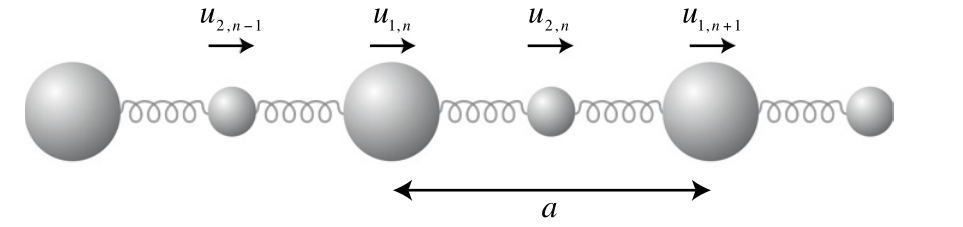
\includegraphics[width=0.9\textwidth]{fig/temp/diatomic.png}
	\caption{Diatomic chain}
	\label{fig:diatomic}
\end{figure}

As a visual aid to these index-heavy equations, Figure \ref{fig:diatomic} illustrates the one-dimensional diatomic chain, which is often used in introductory texts. If we consider only nearest-neighbour interactions and identical springs, the bond-centered harmonic energy can be written

\begin{align*}
	E &= \frac{1}{4} \bm{\Theta} \sum_n 2 \left[ u(1,n) - u(2,n) \right]^2 + \frac{1}{4} \bm{\Theta} \sum_n 2 \left[ u(2,n) - u(1,n+1) \right]^2 \\
	  &= \frac{1}{2} \bm{\Theta} \sum_n \left[ u(1,n) - u(2,n) \right]^2 + \frac{1}{2} \bm{\Theta} \sum_n \left[ u(2,n) - u(1,n+1) \right]^2
\end{align*}

\noindent where the factor of 2 comes from double-counting. The purpose of this example is to show that the (somewhat abstract) harmonic energy in equation \eqref{eq:eharm} is equivalent to our intuitive understanding of coupled harmonic oscillators. 


With this in mind, we can return to the matter at hand and write the equation of motion for an arbitrary atom

\[ m_j \ddot{\bm{u}}(jl, t) = - \frac{\partial E}{\partial u(jl)} = -\frac{1}{2} \sum_{l,\lp} \sum_{j,\jp} \fc u(\jp \lp, t) \, \]

\noindent where $m_j$ is the atomic mass.






